\newpage
\section{Interpreting State Machines [12 points]}\label{sec:interpreting}
Let $\Sigma = \{0, 1\}$.
For each of the following DFAs explain what language they recognize.%\\[0.25cm]


\begin{enumerate}[label=(\roman*)]
\item \textbf{[6 points]}
Please see the DFA of machine $M_1$ below.
\begin{figure}[h]
\begin{center}
{
\psfrag{0}{$0$}\psfrag{1}{$1$}
\psfrag{0,1}{$0,1$}
\psfrag{q0}{$q_0$}\psfrag{q1}{$q_1$}\psfrag{q2}{$q_2$}\psfrag{q3}{$q_3$}
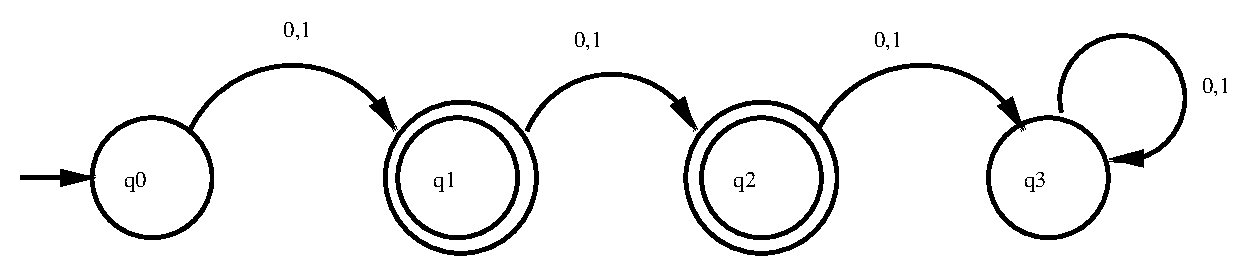
\includegraphics[width=0.5\columnwidth]{figs/dfa2}
}
\end{center}
\end{figure}
For this machine $M_1$, also give its formal description as a 5-tuple. 
You do not need to do this for the machine $M_2$ that follows in part (ii).
\end{enumerate}


\newpage
{\begin{center}\textbf{(continuation of exercise \ref{sec:interpreting})}\end{center}}
\begin{enumerate}[label=(\roman*)]\setcounter{enumi}{1}
\item \textbf{[6 points]}
Please see the DFA of machine $M_2$ below.
\begin{figure}[h]
\begin{center}
{
\psfrag{0}{$0$}\psfrag{1}{$1$}
\psfrag{0,1}{$0,1$}
\psfrag{q0}{$q_0$}\psfrag{q1}{$q_1$}\psfrag{q2}{$q_2$}\psfrag{q3}{$q_3$}
\psfrag{q4}{$q_4$}\psfrag{q5}{$q_5$}\psfrag{q6}{$q_6$}\psfrag{q7}{$q_7$}
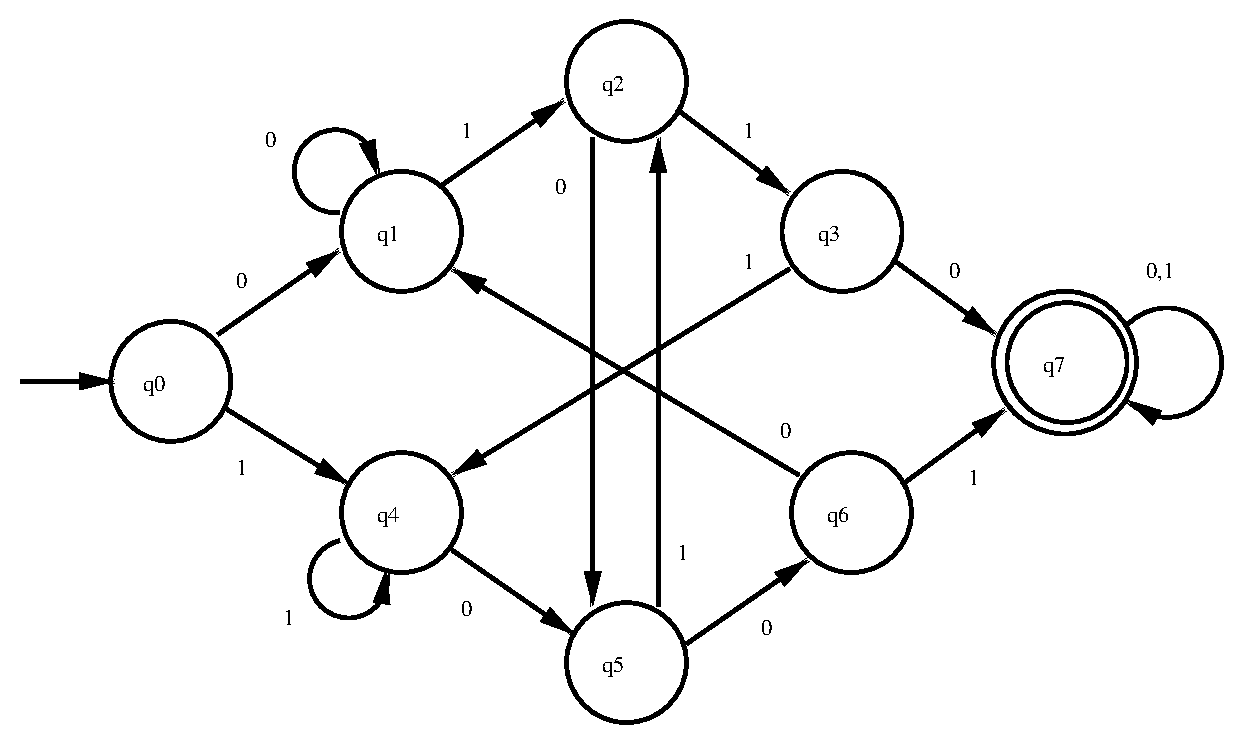
\includegraphics[width=0.5\columnwidth]{figs/dfa3}
}
\end{center}
\end{figure}

\end{enumerate}